\clearpage
\setcounter{page}{1}
\section{Pengertian oracle apex, dan Cara membuat workspace pada oracle apex.}
\begin{document}
Oracle Application Express (APEX) adalah platform yang berfungsi untuk membangun aplikasi yang aman, dengan fitur kelas dunia dan dapat digunakan dimana saja.Apex memiliki tiga alat utama yang digunakan di dalamnya, yakni Application Builder, SQL Qorkshop dan Utility. Berikut ini merupakan penjelasan dari ketiga alat tersebut, di antaranya yakni :
\section{Tutorial Pembuatan Aplikasi}
\paragraph{}
Berikut ini merupakan tata cara pembuatan aplikasi menggunakan oracle apex, di antaranya yaitu :\\
\begin{enumerate}
	\item Sign in ke akun oracle apex anda melalui laman https://apex.oracle.com/pls/apex/f?p=4550:1:107486695866967::::: sehingga akan muncul tampilan seperti berikut ini :
		\begin{figure}[H]
		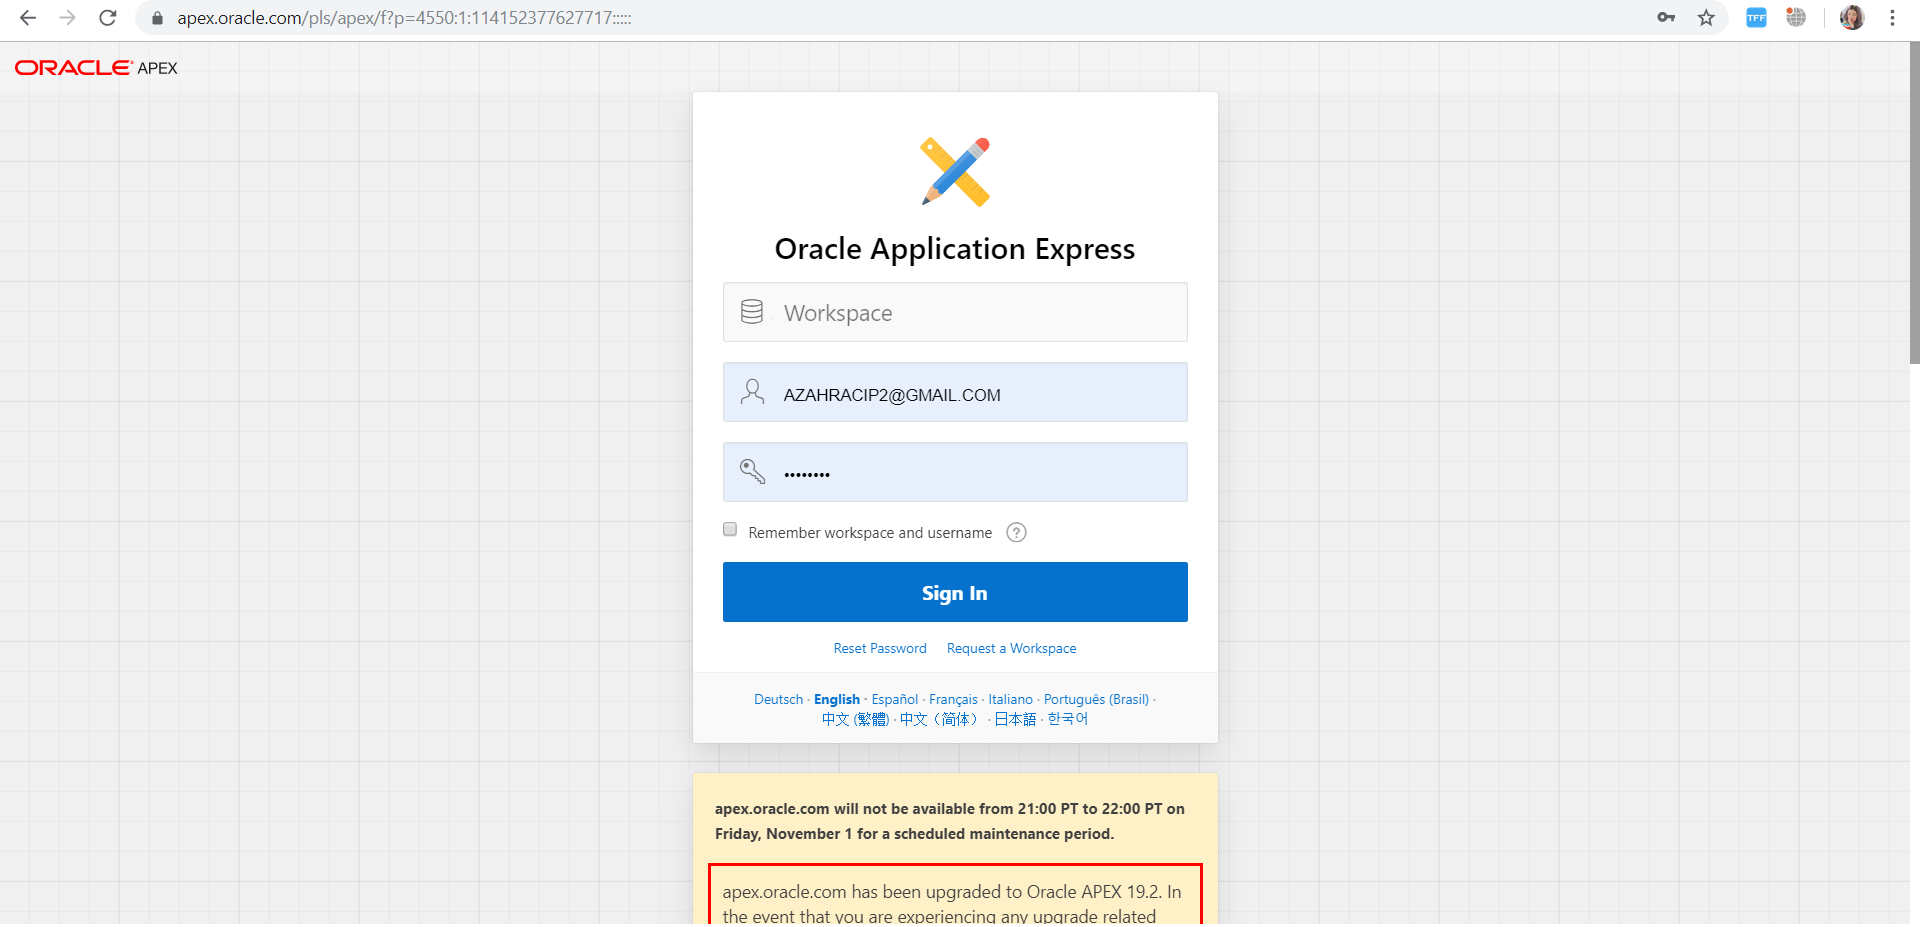
\includegraphics[width=4cm]{figures/signin.png}
		\centering
		\caption{Sign in}
		\end{figure}
	\item Setelah anda masuk ke akun apex anda, maka akan muncul tampilan seperti berikut
		\begin{figure}[H]
		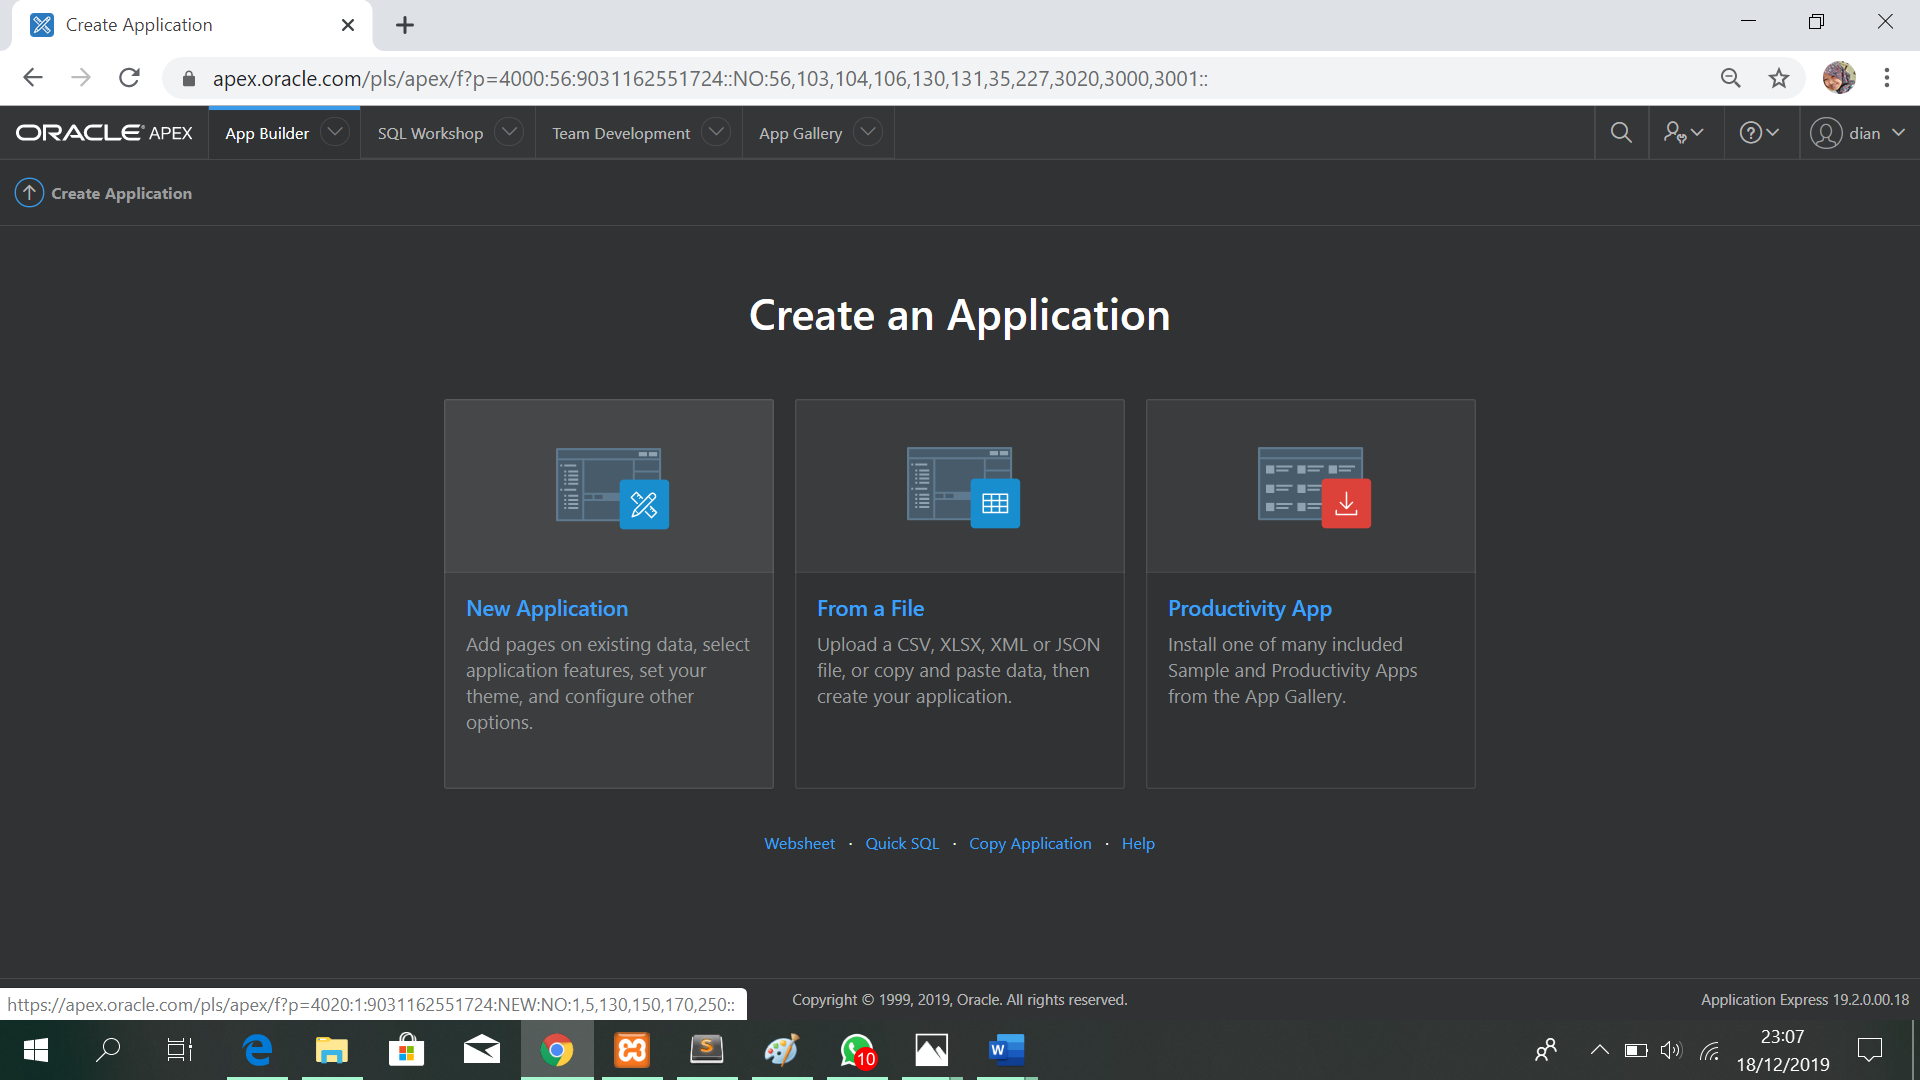
\includegraphics[width=4cm]{figures/2.png}
		\centering
		\caption{Tampilan Awal}
		\end{figure}
	\item Setelah itu, normalisasikan data yang akan anda masukkan ke dalam apex, berikut ini merupakan data akademik mahasiswa teknik informatika politeknik pos indonesia sebelum dinormalisasikan
				\begin{figure}[H]
				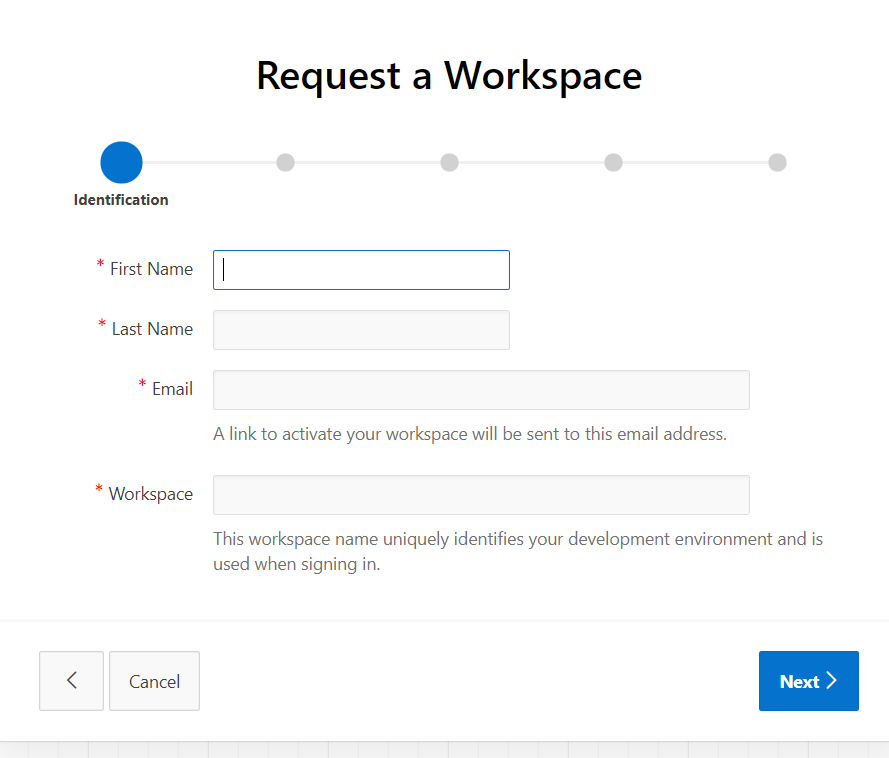
\includegraphics[width=8cm]{figures/3.png}
				\centering
				\caption{Data sebelum dinormalisasi}
				\end{figure}
		Setelah itu, kita hilangkan judul di bagian atasnya dengan mendelete dan begitu pula pada kolom nomor. Sehingga menjadi seperti berikut. 
				\begin{figure}[H]
				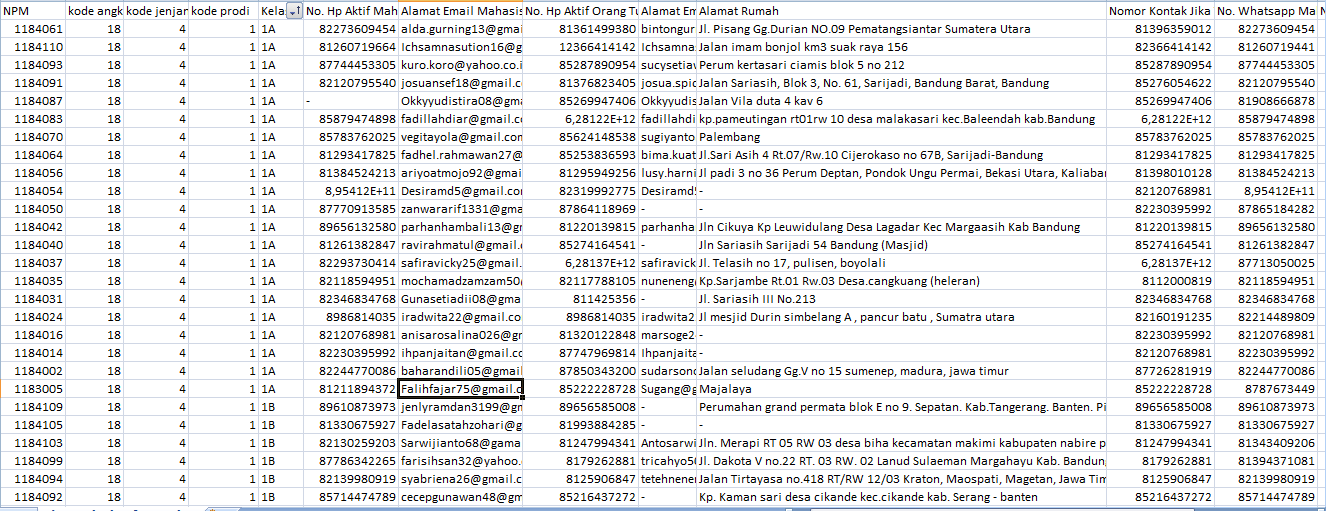
\includegraphics[width=8cm]{figures/normalisasi.png}
				\centering
				\caption{Data setelah dinormalisasi}
				\end{figure}
	\item Di sisi lain. buatlah file excel baru yang memuat kode unik yang merupakan primary key dari tabel tersebut.
				\begin{figure}[H]
				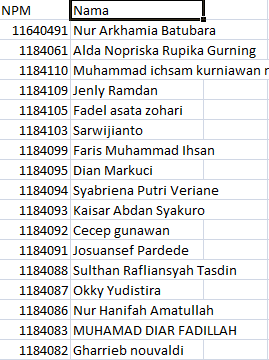
\includegraphics[width=8cm]{figures/npm.png}
				\centering
				\caption{Contoh file tabel npm}
				\end{figure}
			Lakukan hal yang sama pada tabel yang dinormalisasikan. Disini saya membuat tabelprodi, tabeljenjang, tabelangkatan, tabelnpm, dan tabeldatamahasiswa
	\item Kemudian klik menu app builder pada apex, setelah itu akan muncul tampilan seperti berikut dan pilihlah 'Create'
				\begin{figure}[H]
				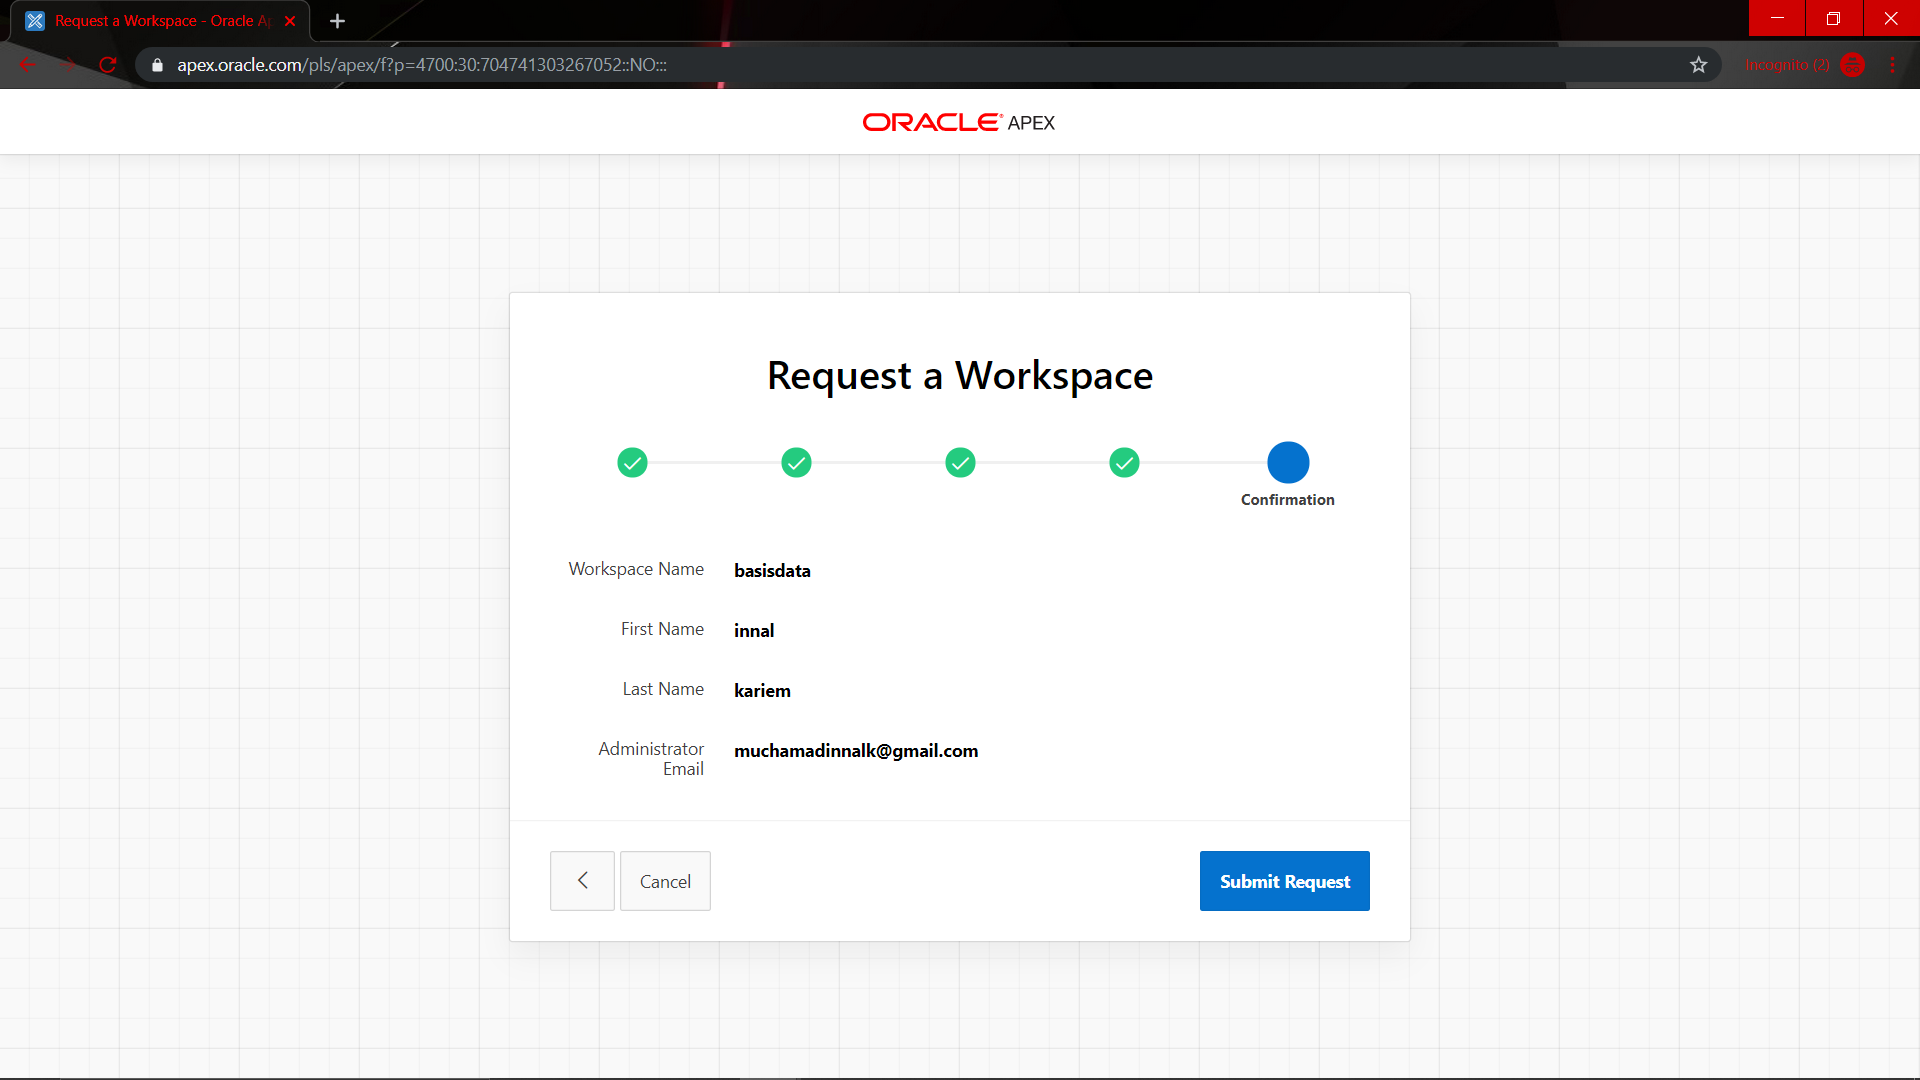
\includegraphics[width=8cm]{figures/5.png}
				\centering
				\caption{Tampilan App Builder}
				\end{figure}
	\item Setelah itu pilih add from file untuk memasukkan data yang telah tersedia sebelumnya. Pastikan anda menyimpan file excel tersebut dengan format .csv atau .xlsx
	\item Setelah itu anda akan ditampilkan pada laman load data, anda dapat men-drag atau mengklik 'choose file' untuk memasukkan file tersebut
				\begin{figure}[H]
				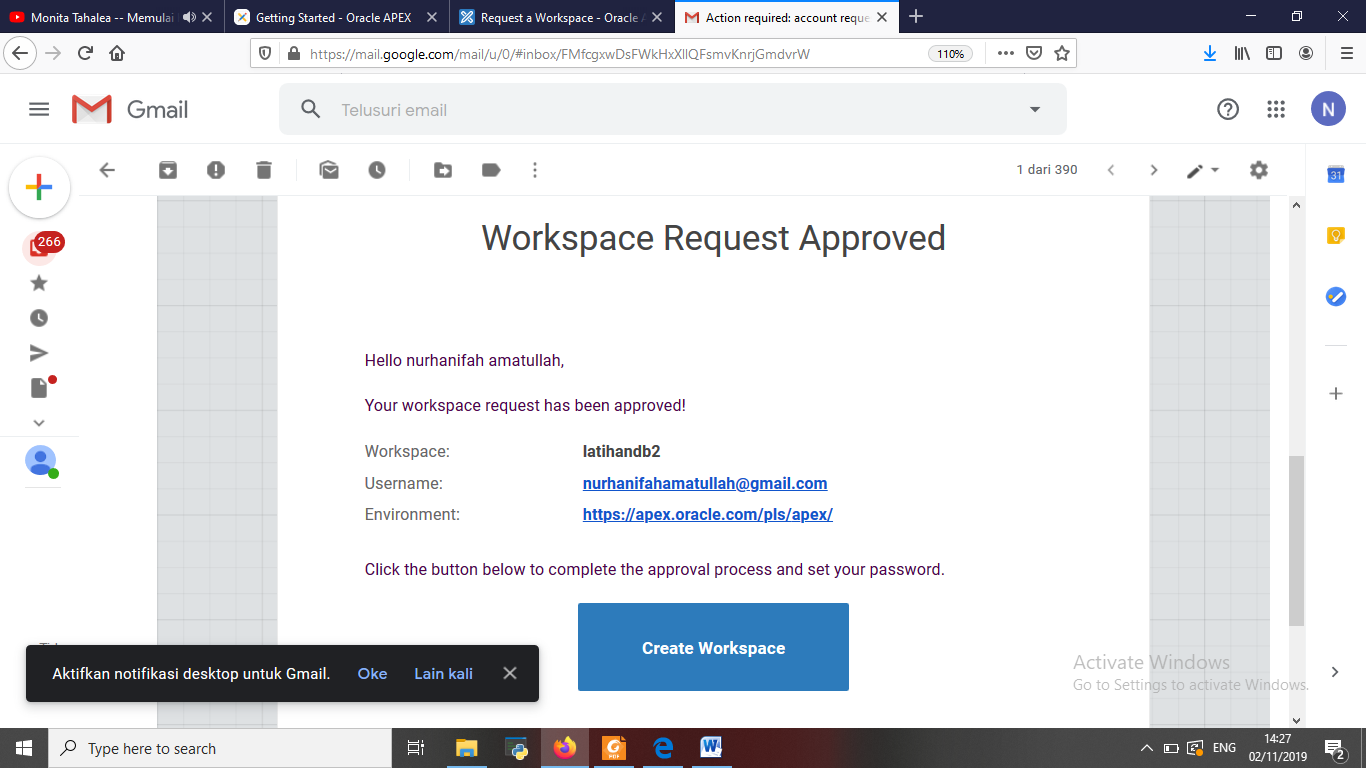
\includegraphics[width=8cm]{figures/6.png}
				\centering
				\caption{Drag file yang akan diinputkan}
				\end{figure}
	\item Setelah file diupload, lalu klik configure untuk memastikan data. Setelah data sudah benar, kemudian klik "Save Changes". Lalu load data.
				\begin{figure}[H]
				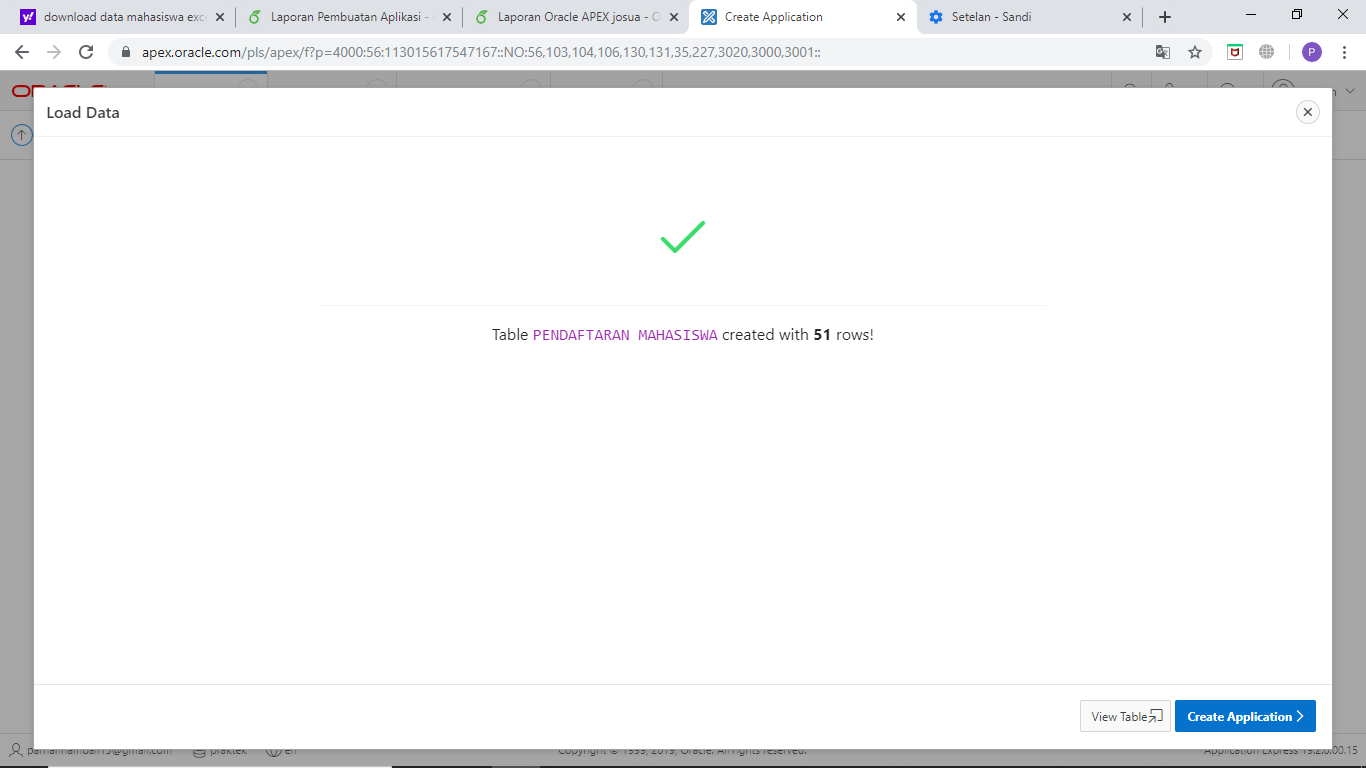
\includegraphics[width=8cm]{figures/8.png}
				\centering
				\caption{Konfigurasi data}
				\end{figure}
	\item Setelah data masuk, maka akan muncul tampilan seperti berikut ini, kamudian exit terlebih dahulu, jangan langsung menekan tombol create application.
				\begin{figure}[H]
				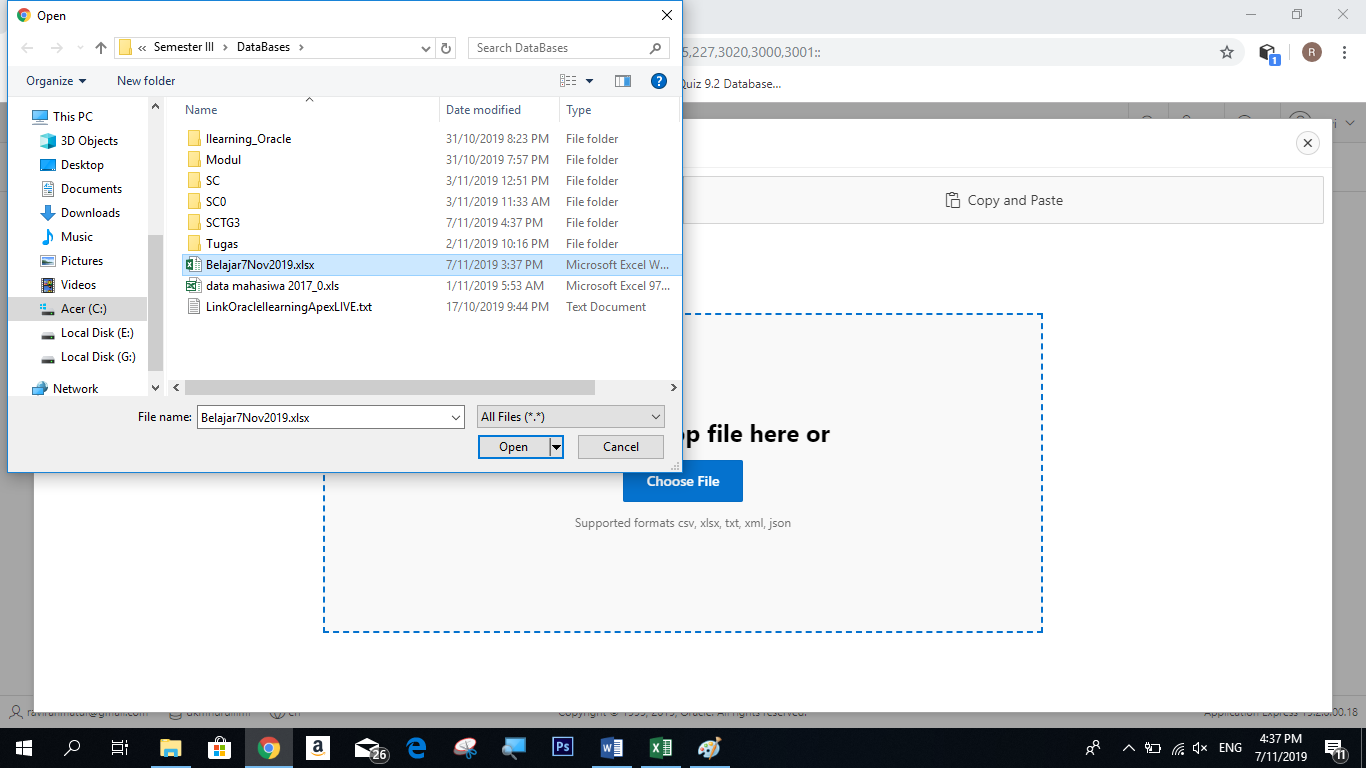
\includegraphics[width=8cm]{figures/9.png}
				\centering
				\caption{Data telah diinput}
				\end{figure}
	\item Lalu, ulangi tahapan tadi dengan memasukkan file tabeljenjang,tabelprodi,tabelangkatan, tabelnpm, dan datamahasiswa.
	\item Setelah data mahasiswa telah diload, kemudian pilih "create application". Lalu akan muncul tampilan seperti berikut
				\begin{figure}[H]
				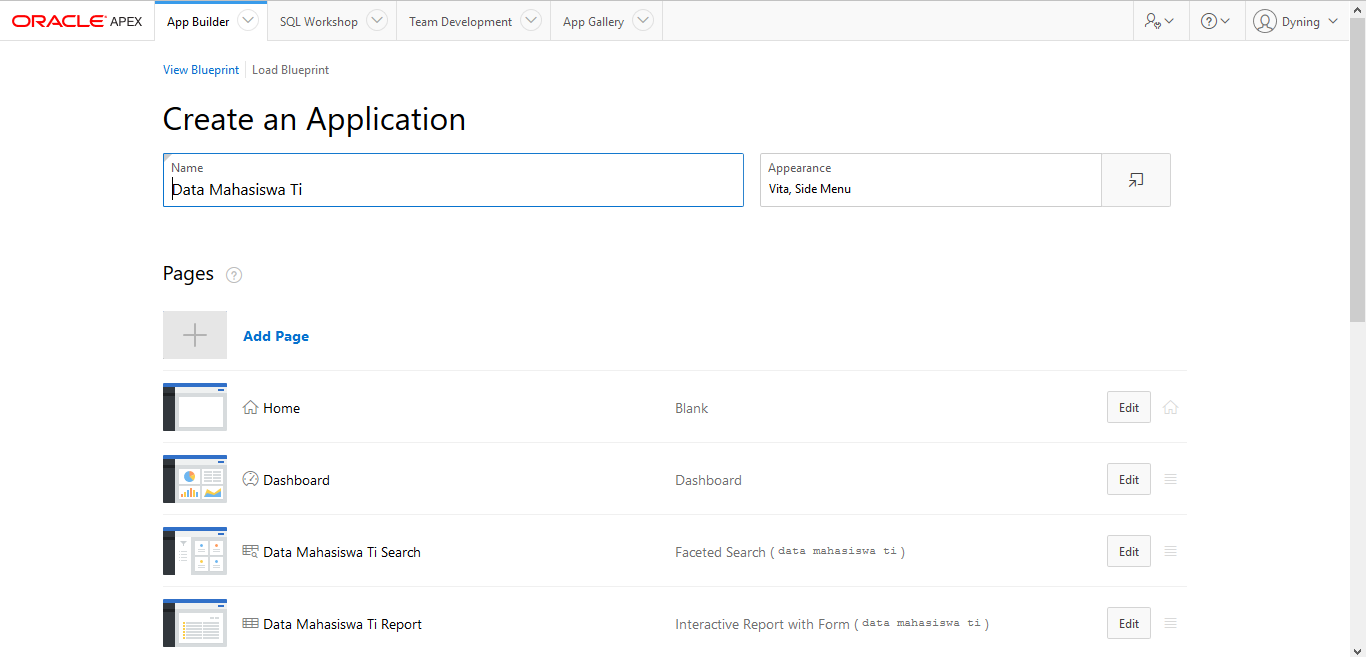
\includegraphics[width=8cm]{figures/createap.png}
				\centering
				\caption{Tampilan setelah diload}
				\end{figure}
	\item Pilih Add Page, kemudian pilih Interactive Report
		\begin{figure}[H]
				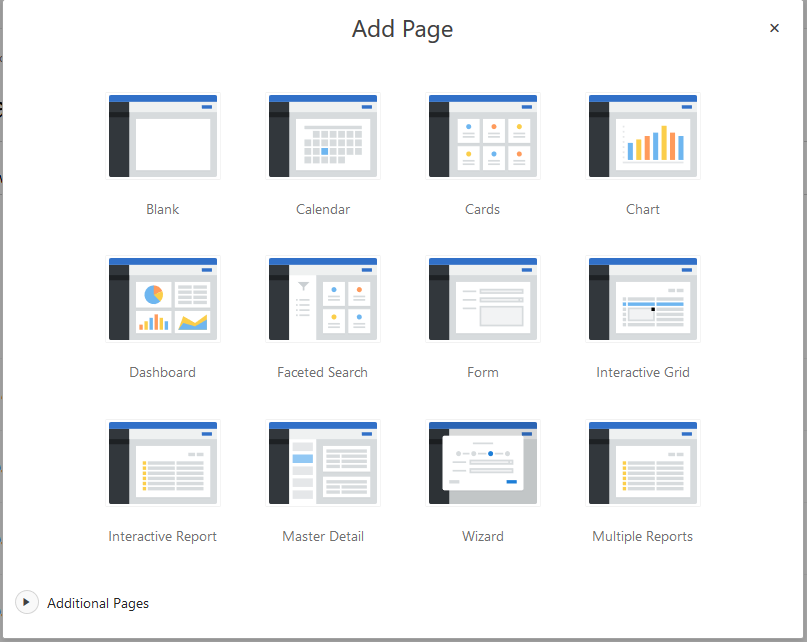
\includegraphics[width=8cm]{figures/addpage.png}
				\centering
				\caption{Penggunaan Interactive Report}
				\end{figure}
	\item Lalu isikan Report Page sesuai yang anda inginkan, lalu masukkan tabel yang diinginkan
				\begin{figure}[H]
				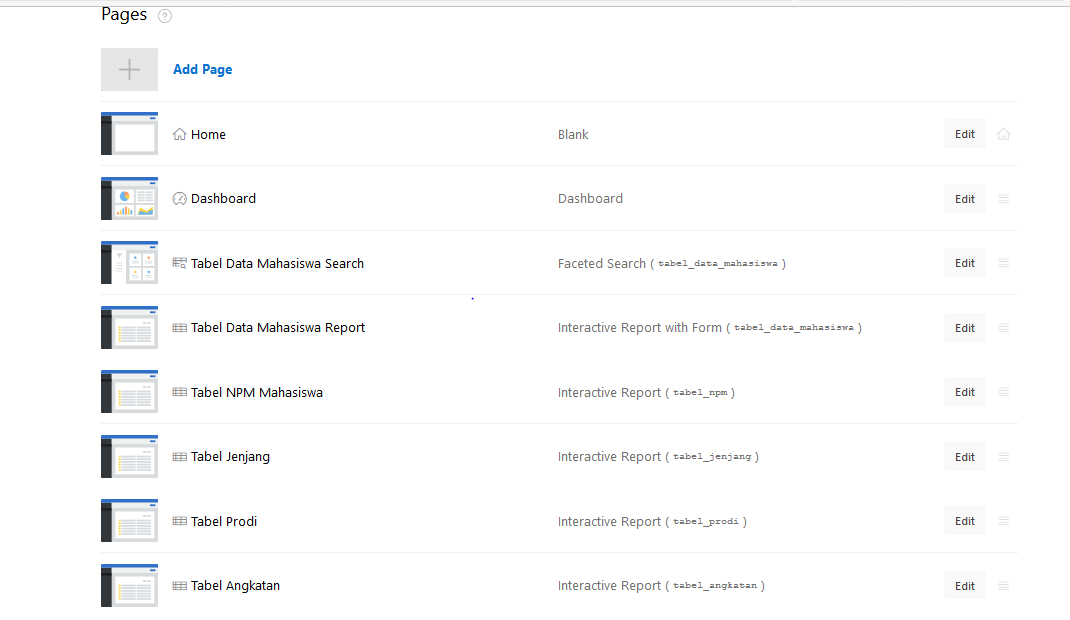
\includegraphics[width=8cm]{figures/addpage2.png}
				\centering
				\caption{Tampilan penambahan page}
				\end{figure}
	\item Create Application
				\begin{figure}[H]
				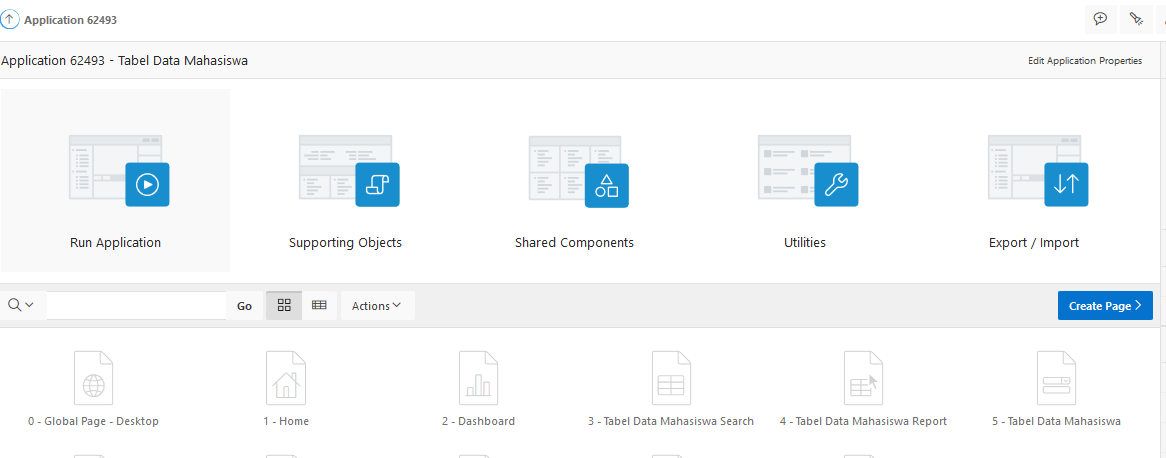
\includegraphics[width=8cm]{figures/setelah.png}
				\centering
				\caption{Tampilan psetelah aplikasi dibuat}
				\end{figure}
	\item Lalu ke menu SQL Workshop dan pilih object browser
	\item Pilih tabel datamahasiswa kemudian hapus kolom ID dengan menekan 'drop columns'. Lalu akan muncul tampilan seperti berikut.
				\begin{figure}[H]
				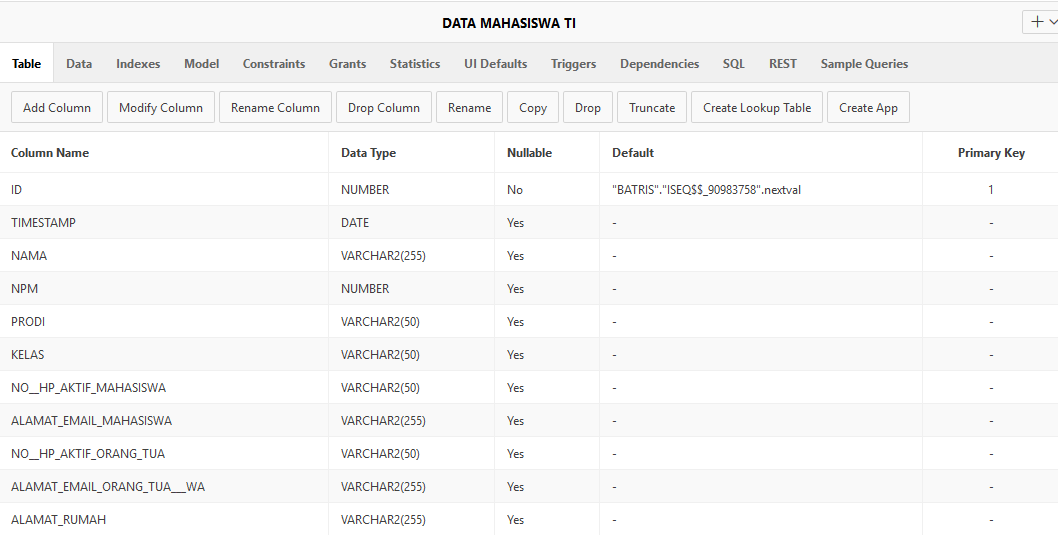
\includegraphics[width=8cm]{figures/datati.png}
				\centering
				\caption{Menghapus kolom yang ID}
				\end{figure}
	Klik next, lalu finish.
	\item Lakukan hal yang sama pada tabelkodenpm, tabelangkatan, tabeljenjang, dan tabelprodi
	\item Pastikan menggantikan nama table yang memiliki spasi dengan digantikan menggunakan underscore. Contoh data mahasiswa diganti menjadi data(underscore)mahasiswa
	\item Pada menu SQL Workshop, pilih SQL Command.
	\item Ketikkan kode sebagai berikut\\
	            \begin{figure}[H]
				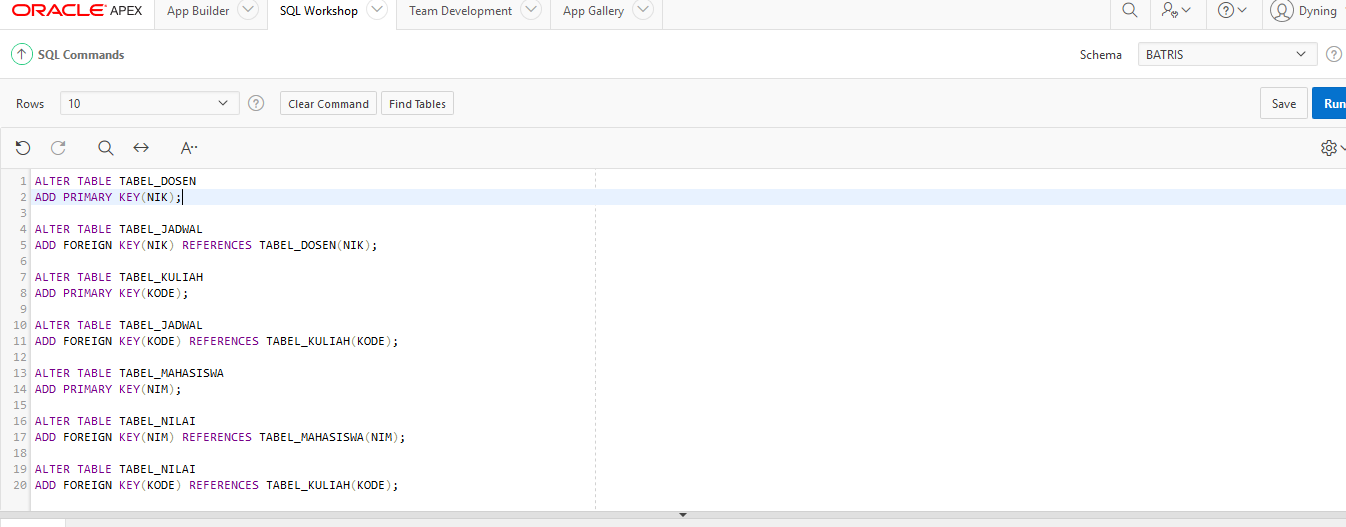
\includegraphics[width=8cm]{figures/kode.PNG}
				\centering
				\caption{kode yang diketikkan}
				\end{figure}
	Untuk menjalankan per bagian, blok bagian yang akan dijalankan terlebih dahulu, kemudian klik tombol run
	\item Setelah itu, cek apakah setiap tabel telah memiliki primary key atau belum dengan mengetikkan sebagai berikut :\\
                \begin{figure}[H]
				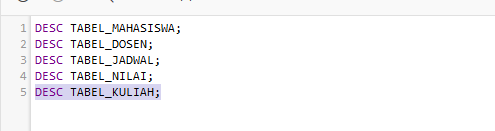
\includegraphics[width=8cm]{figures/kode2.png}
				\centering
				\caption{kode untuk mengecek status}
				\end{figure}
	\item Jalankan aplikasi yang telah dibuat sebelumnya. Maka tampilan aplikasinya akanmenjadi seperti berikut ini
				\begin{figure}[H]
				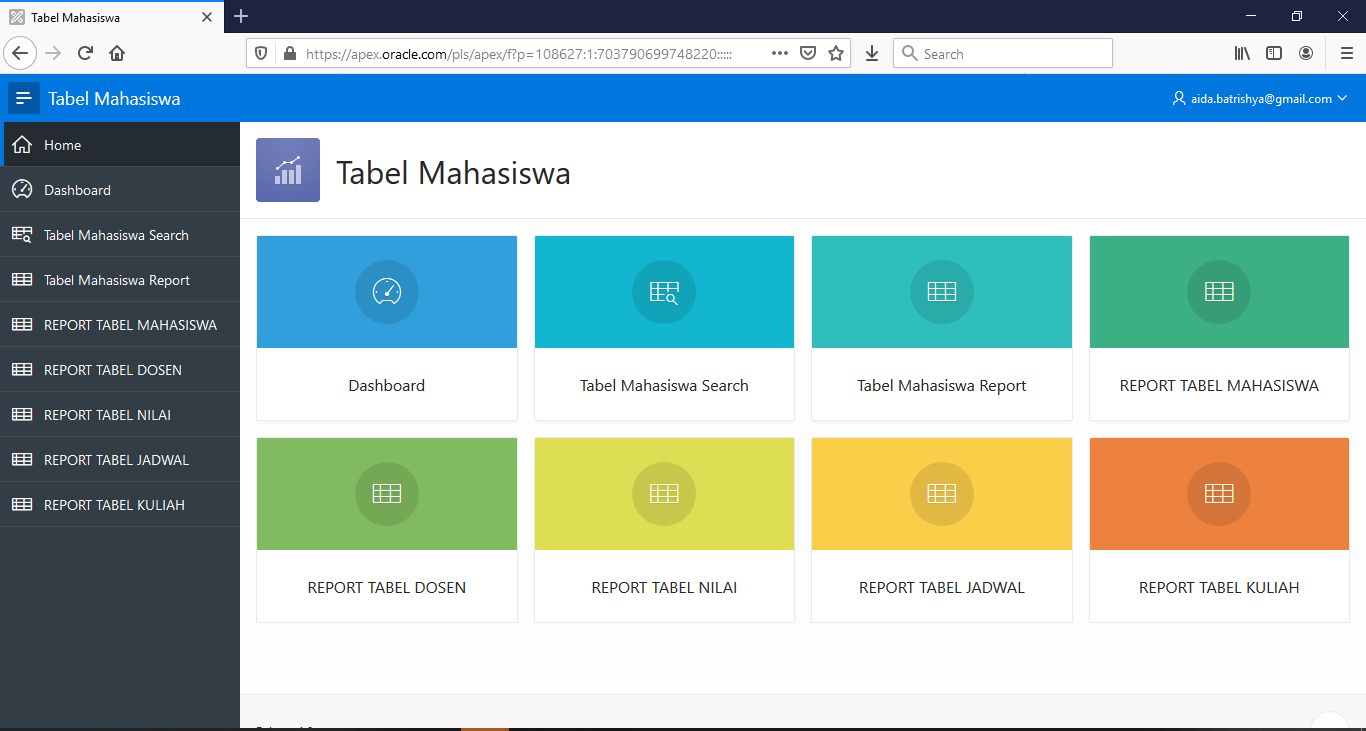
\includegraphics[width=8cm]{figures/aplikasi.png}
				\centering
				\caption{contoh aplikasi}
				\end{figure}
\end{enumerate}
\end{document}